%================ch2======================================
\chapter{Preprocessing the data}\label{ch:ch2}

\section{Acquiring the data}
Initially the data from Gaia is queried from the VizieR database \citep{vizier}. The results obtained by Cantat-Gaudin \citep{cg} can be obtained in a tabular form. Hence we obtain the data for 1229 clusters. The database enables us to access position, motion, cataloguing and color information. We require only the photometric data - the color magnitude and the photometric magnitude for the first part. This data was scraped from the website. This enables us to plot a color magnitude diagram for all the clusters. The probablity of being a member was also considered and the clusters with a probability of more than $0.7$ were marked with larger points. The plots of these clusters were analysed, and ten clusters (IC 4651, IC 4756, NGC 752, NGC 1664, NGC 2281, NGC 2287, NGC 2527, NGC 6281, NGC 6405, NGC 6475) were shortlisted for further analysis.


\begin{figure}[h]
 \centering
 \begin{subfigure}[b]{0.45\textwidth}
   \centering
   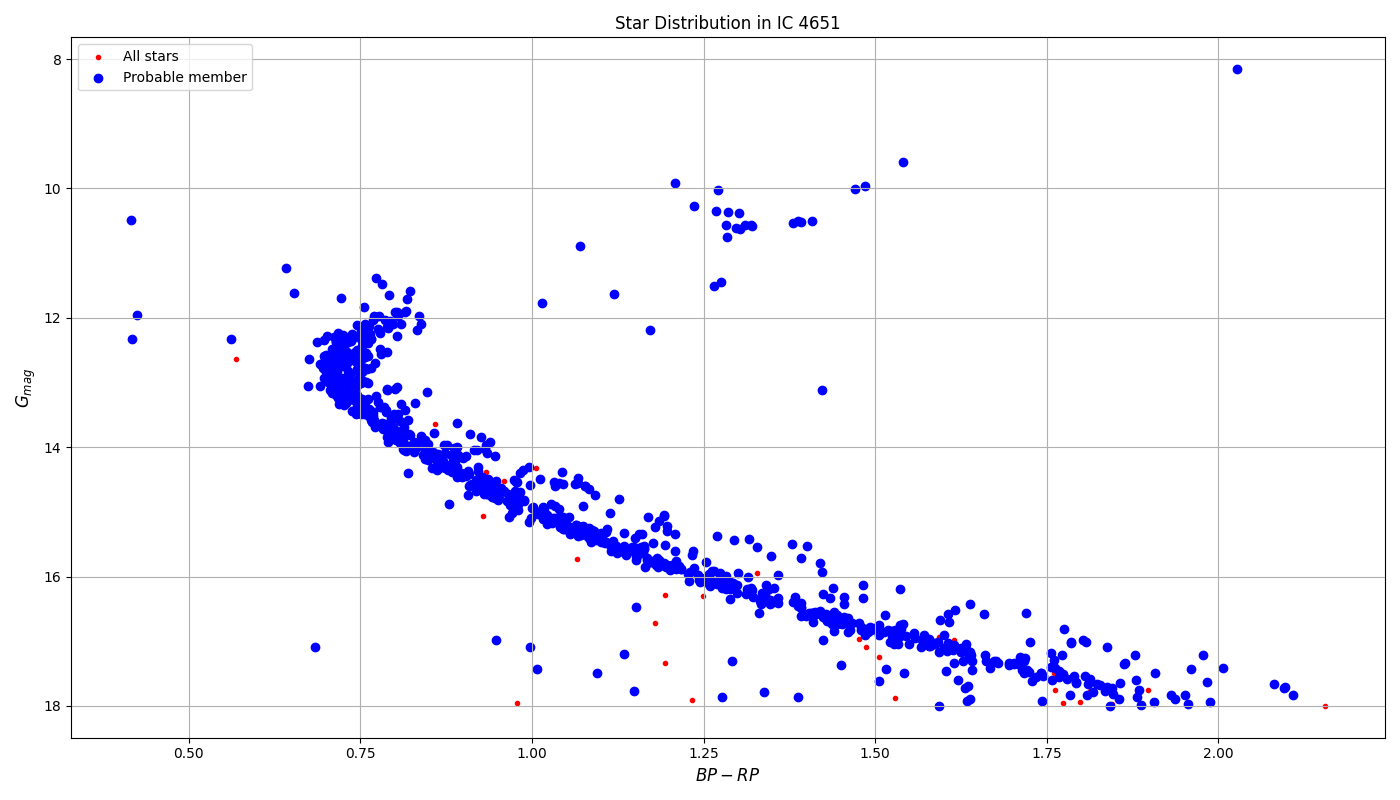
\includegraphics[width=\textwidth]{IC 4651.png}
   \caption{IC 6451}
   \label{fig:im1}
  \end{subfigure}
 ~
 \begin{subfigure}[b]{0.45\textwidth}
   \centering
   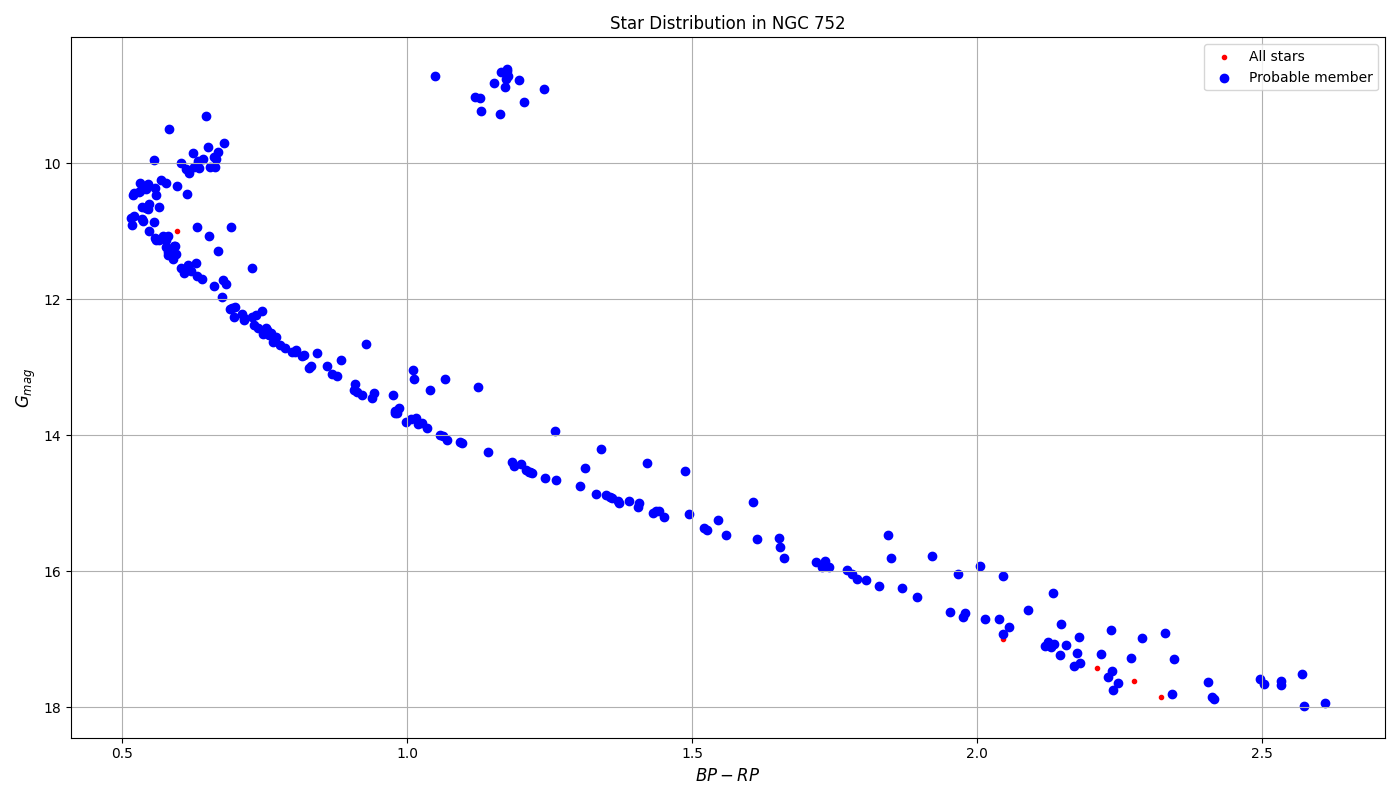
\includegraphics[width=\textwidth]{NGC 752.png}
   \caption{NGC 752}
   \label{fig:im2}
 \end{subfigure}
 \caption{CMD for star clusters}
 \label{fig:subfigs_cap1}
\end{figure} 


 
 